\section{Çin Odası Testi}
1980'lerde Amerikalı felsefeci John Searle tarafından ortaya atılmıştır. Turing Testini geçebilen bir makinenin hiçbir şekilde düşünüp anlama yeteneğine sahip olmayacağını savunmuştur. Bunun için Çin Odası Paradoksunu önermekteydi. Çin Odası Paradoksu senaryosunda, Çince bilmeyen bir kişi Çin Odası adında kapalı bir odada bulunmaktadır. Odanın içinde üzerinde Çince yazılar yazılmış tabelalar ve bu tabelaları açıklayan bir kural kitabı bulunur. Kural kitabı, Çince'yi tamamen söz dizimlerine göre açıklamaktadır. Bunlara yanıt olarak odadaki kişinin uygun tabelayı dışarı vermesi beklenir.  Dışarıdaki gözlemciye göre, bu kişi Çince bilmekteymiş gibi görünmektedir, çünkü dışarıdaki gözlemci, kişinin verdiği cevapları Çince karakterlerle yazılmış metne uygun olduğunu doğrular. Searle, bu senaryo üzerinden yapay zekanın bilinçli bir zekaya sahip olup olmadığı konusunda bir argüman geliştirir. Ona göre, bu kişi Çince karakterlerle yazılan metni işlerken, gerçekte anlamını anlamamaktadır. O sadece talimatları izleyerek sembolik bir işlem yürütmektedir. Bu nedenle, Searle'a göre, bu tür sembolik işlemleri yapan bir makine de gerçek bir zeka veya bilinç sahibi olamaz.

\begin{figure}[h]
    \centering
    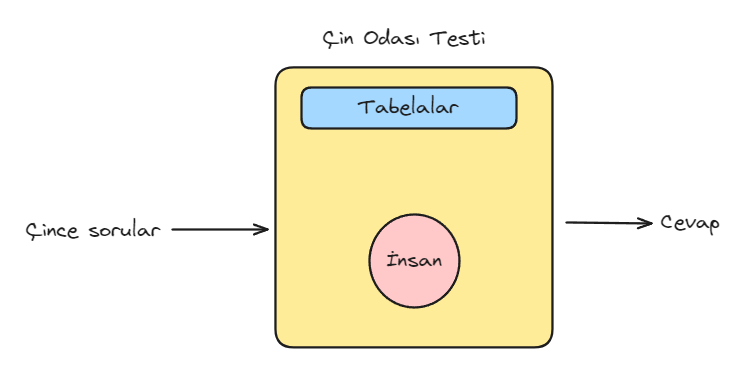
\includegraphics[width=1\textwidth]{images/chinese_room_test.png}
    \caption{Çin odası testi.}
    \label{fig:enter-label}
\end{figure}

\newpage
